\documentclass[a4paper]{article}
%% Language and font encodings
\usepackage[english]{babel}
\usepackage[T1]{fontenc}
\usepackage{graphicx}
\usepackage{float}
\usepackage{amsmath}
\usepackage{amssymb}
\usepackage[colorinlistoftodos]{todonotes}
\usepackage[colorlinks=true, allcolors=blue]{hyperref}
\usepackage{xcolor}

%% Sets page size and margins
\usepackage[a4paper,top=3cm,bottom=2cm,left=3cm,right=3cm,marginparwidth=1.75cm]{geometry}

\title{
\includegraphics[width=0.6\textwidth]{images/logo_polimi_scritta.eps}\\[1em]
    HOP-PAAL: A Formal Frogger Journey\\[0.4em]
    \normalsize \text{Formal Methods for Software Engineering}\\
    \normalsize \text{A.Y. 2025-2026}}
\author{Daniele Crippa, Dario Cambi and Giorgio Ciraci \\[0.8em]
    \normalsize \text{Politecnico di Milano}\\
    \small \textit{daniele5.crippa@mail.polimi.it}\\
    \small \textit{dario.cambi@mail.polimi.it}\\
    \small \textit{giorgio.ciraci@mail.polimi.it}\\}



\date{}
\begin{document}
\maketitle

\begin{abstract}
UPPAAL is a tool for modeling, simulating, and verifying real-time systems as networks of Timed Automata. In this report, we present the modeling and formal verification of a simplified version of Frogger, a classic arcade game. Both a vanilla and a stochastic version of the model are developed and analyzed.
\end{abstract}
\newpage
\section{Introduction}
\textbf{Frogger} is a classic arcade video game released in 1981, one of the most iconic titles of its era. The primary goal of the game is to successfully guide a frog into a \textbf{home bay} as many times as possible, requiring the player to cross a \textbf{busy highway} and a \textbf{dangerous river}, avoiding moving cars and jumping on logs and turtles to avoid falling into the water.

\textbf{Formal verification} is a technique used to \textbf{prove or disprove the correctness of a system} with respect to a formal specification. While commonly applied to \textbf{hardware and safety-critical software}, it can also be used to model and verify the behavior of more unconventional systems, such as video games, which are rarely formally defined.

\textbf{UPPAAL} is a tool designed for \textbf{modeling, simulating, and verifying real-time systems} using networks of \textbf{Timed Automata}. It provides a graphical interface alongside a powerful \textbf{query language} that allows the user to formally check properties on the system.

In this project, UPPAAL is applied to \textbf{model and formally verify} a simplified version of Frogger, covering all its \textbf{core mechanics} as defined in the specifications. The goal is to demonstrate that the model \textbf{behaves correctly under all possible conditions}, using both a \textbf{vanilla} and a \textbf{stochastic} version of the automata network.

\subsection{Assumptions and further clarifications}
The following assumptions are made on the specifications:
\begin{itemize}
    \item One time unit in UPPAAL corresponds to 0.1 seconds
    \item Between any two consecutive moves of Frogger, at least 1 time unit must elapse; this prevents unrealistic Zeno behaviors
    \item The game timer is assumed to start when Frogger respawns, ignoring the 
    respawn cooldown. As a consequence, the last playable run starts with a game 
    timer of 2 seconds, during which Frogger is bound to die, since the respawn 
    cooldown and the game timer are both equal to 2 seconds.
    \item The initial level is zero.
\end{itemize}

After further context clarifications with the professor we also defined the following edge cases or ambiguous situations:
\begin{itemize}
    \item 
\end{itemize}

\newpage
\section{Model Description}
The model is based on 4 primary components:
\begin{itemize}
    \item \textit{Frogger}
    \item \textit{Vehicle Lane}
    \item \textit{Floating Lane}
    \item \textit{Diving Turtles Manager}
\end{itemize}

\subsubsection*{Frogger}
The protagonist of the game, it starts with 5 lives and must reach all 5 home bays to complete a level. The frog dies upon collision with a vehicle, contact with open water, or expiration of the time limit.

\subsubsection*{Vehicle Lane}
Models a road lane populated by moving vehicles of varying speed and size. 
Each lane defines a fixed direction of travel, and a collision with the frog results in the loss of a life.

\subsubsection*{Floating Lane}
Models a river lane composed of floating objects, such as logs and turtles. 
When the frog stands on a floating object, it is carried along with it. 
Landing on an empty water cell results in immediate death.

\subsubsection*{Diving Turtles Manager}
Manages the submersion cycle of diving turtles, cycling through the states 
\textit{Emerged}, \textit{Diving}, \textit{Submerged}, and \textit{Emerging}. 
When turtles submerge, a broadcast signal notifies the Floating Lane, 
which treats the occupied cell as open water, causing the frog to die if standing on it.


\subsection{Overall Design Choices}
Before describing each template in detail, we summarise the main design 
choices that shape the whole model and that are shared across its components.

\subsubsection*{Game Map}
The game map is encoded as a fixed matrix of size \texttt{GRID\_H}$\times$\texttt{LANE\_W}, 
where each cell holds its initial logical content. A central choice is that moving objects are \textit{never} 
physically rewritten in this matrix: their motion is represented by a single 
per-lane shift variable inside the lane templates. This keeps the 
representation compact and avoids continuously updating a large array, which 
would otherwise enlarge the state space.

\subsubsection*{Lane Abstraction}
Roads and rivers are both modelled as lanes, since they share most of their 
logic; this avoids modelling each element separately and prevents the state 
space from exploding. The motion of objects is not rewritten in the map matrix 
but represented by a single per-lane shift variable, keeping the 
representation compact.

The logical lane width \texttt{LANE\_W} is intentionally larger than the 
visible grid \texttt{GRID\_W} (20 against 18): the two extra off-screen cells 
model the re-entry delay required by the specification, so that an object 
leaving the map does not reappear immediately on the other side. For the same 
reason, \texttt{frog\_x} ranges over the full \texttt{LANE\_W}, allowing 
Frogger to be carried slightly off-screen while riding a floating object.

\subsubsection*{Lanes Handle Frogger's Death}
The decision to kill Frogger is delegated to the lanes rather than to the frog 
itself. Each lane knows the global position of Frogger, so it is 
the natural place to detect a collision or an unsafe cell; when this happens, 
it requests the death through the \texttt{kill\_frog} channel, which 
\textbf{Frogger} automaton consumes by removing a life and respawning. This keeps 
the collision logic local to each lane and leaves the frog simple and focused on its own movement and life management.

\subsubsection*{Turtles Management}
The global submersion cycle of the diving turtles is delegated to a separate template,
so that the shared timing is defined in one place and simply observed by the lanes.

Moreover, the water gaps between turtles of the same group are encoded as turtle cells, since Frogger 
standing on those cells is equally safe, the two are semantically equivalent.

\subsection{Frogger}
The frogger template contains the main logic of the frog, including its movement, life management and points assignment.
\begin{figure}[H]
    \centering
    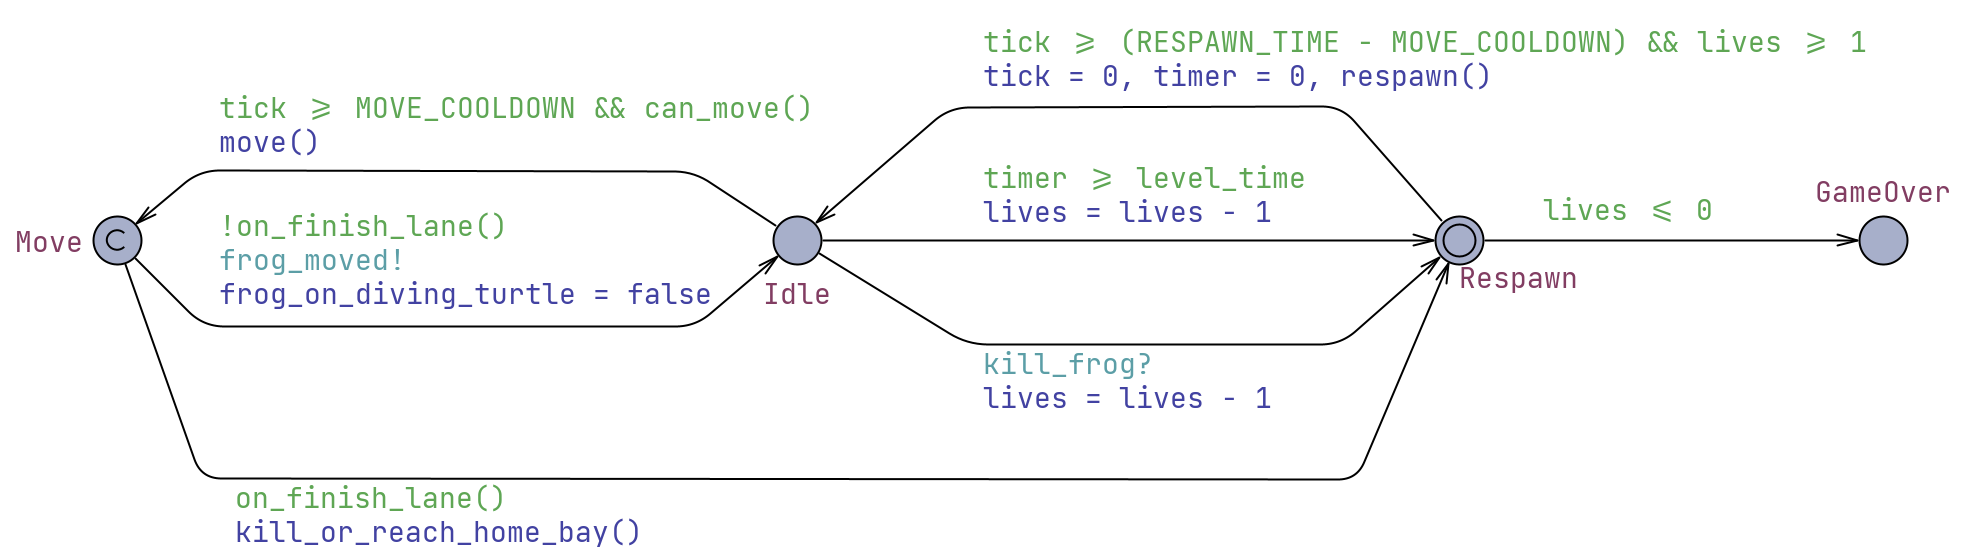
\includegraphics[width=\textwidth]{images/frogger.png}
    \caption{Frogger Template}
    \label{fig:froggerImage}
\end{figure}
The design was made around its possible states: 
\begin{enumerate}
    \item \textbf{Idle} is the central state where the frog is waiting between actions. 
    Three transitions can fire from here: if the move is legal and the cooldown time is over, 
    the frog can go to the \textbf{Move} state; it can be killed either by another template through 
    the \texttt{kill\_frog} channel or by running out of time, losing a life and sending it to the \textbf{Respawn} state.
    
    \item \textbf{Move} is a \textit{committed} state in which Frogger enters after a movement command;
    here, immediately is determined the outcome of its move. If it lands on a finishing 
    lane, it resolves whether a home bay is reached through; otherwise it simply update the position of Frogger 
    and returns to \textbf{Idle}.
    
    \item \textbf{Respawn} is reached whenever the frog loses a life or reaches an home bay. 
    From here, if at least one life remains, the frog waits for the respawn timing and then returns 
    to \textbf{Idle}. If \texttt{lives <= 0}, it transitions to \textbf{GameOver} instead.
    
    \item \textbf{GameOver}: the final state of the automaton, entered when the frog has no lives left.
\end{enumerate}

\subsection{Vehicle Lane}
The vehicle lane template models a single lane of the road, 
populated by vehicles that move at the same speed and share 
the same size; both parameters are constants and defined at the 
instantiation of the template.
\begin{figure}[H]
    \centering
    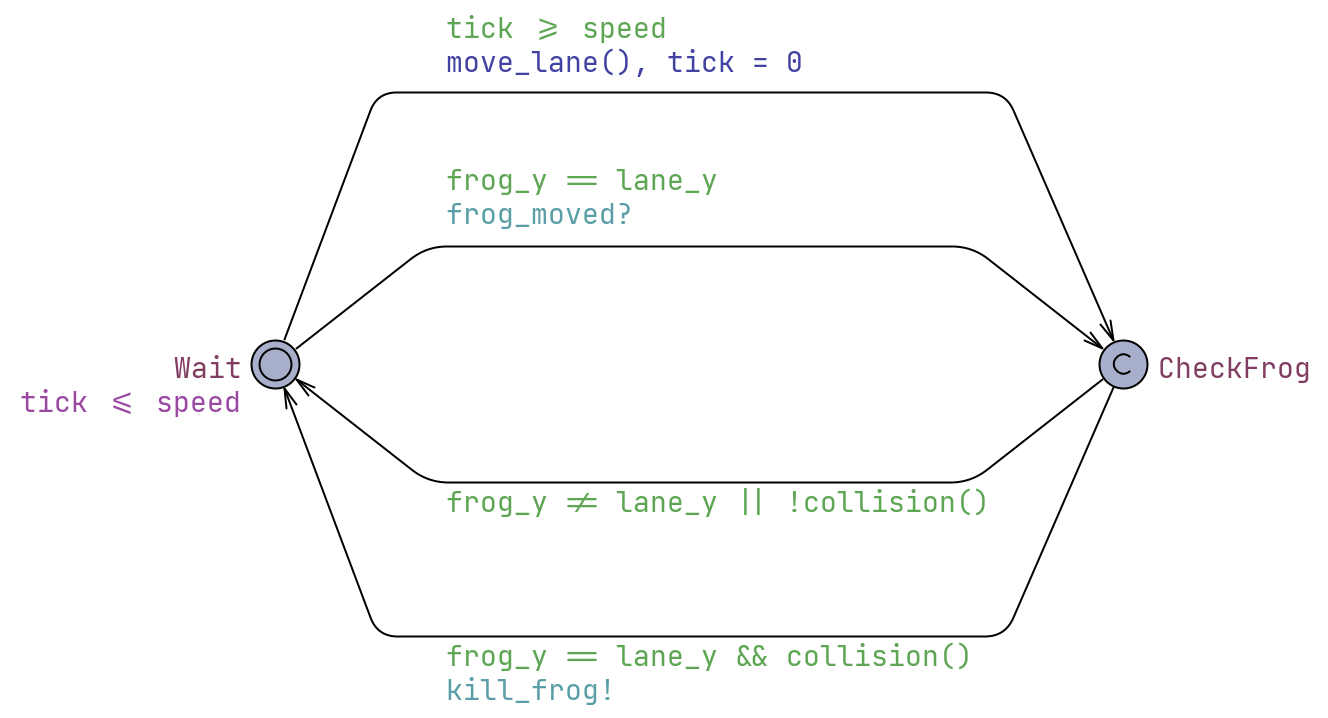
\includegraphics[width=\textwidth]{images/vehicle_lane.png}
    \caption{Vehicle Lane Template}
    \label{fig:vehicleLaneImage}
\end{figure}
The template is realised through two states, \textbf{Wait} and 
\textbf{CheckFrog}. In \textbf{Wait}, the lane lets time pass until 
the interal clock reaches the speed; 
when this happens, it shift the vehicles with the function 
\texttt{move\_lane()}, resets the timer, and transitions to 
\textbf{CheckFrog}. This is a \textit{committed} state, so the 
collision check is performed instantaneously: if a vehicle occupies 
Frogger's position, it signals the death through the \texttt{kill\_frog}
channel and returns to \textbf{Wait}; otherwise it returns to 
\textbf{Wait} without sending any signal.

A second path into \textbf{CheckFrog} is triggered when the frog moves:
the lane is notified through the \texttt{frog\_moved} channel, 
allowing it to verify immediately whether the frog's new position 
is occupied by a vehicle; if so it signals it through the channel
\texttt{kill\_frog}.

\subsection{Floating Object Lane}
The floating lane template models a river lane, where the frog can 
only survive by standing on floating objects, such as logs and turtles.
\begin{figure}[H]
    \centering
    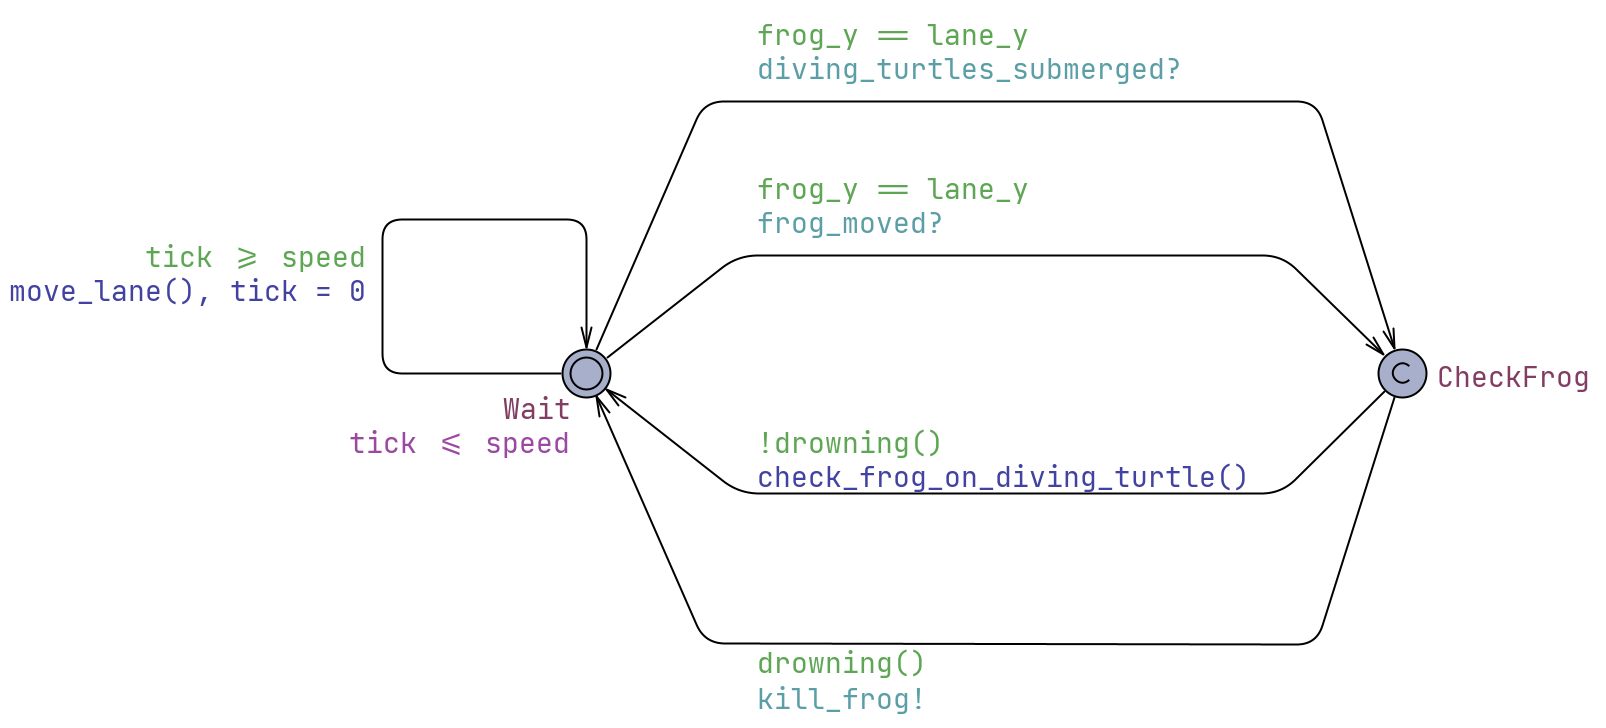
\includegraphics[width=\textwidth]{images/floating_lane.png}
    \caption{Floating Object Lane Template}
    \label{fig:floatingLaneImage}
\end{figure}
The template is structured in two main states, \textbf{Wait} and 
\textbf{CheckFrog}. In \textbf{Wait}, the lane lets time pass until 
the internal clock reaches the speed of the lane; when this happens, 
it shifts the floating objects with the function \texttt{move\_lane()} 
and transitions to \textbf{CheckFrog}. If the frog is currently standing 
on a floating object, its global position is updated within the same 
function, so that it is carried along with the object.

\textbf{CheckFrog} is a \textit{committed} state where the lane verifies 
whether the frog is safe, and it can be reached through three different 
paths. The first is the periodic movement just described: after shifting, 
the lane checks if the frog is drowning with the function \texttt{drowning()}, 
and if it not, it safely returns to \textbf{Wait}; 
otherwise it signals the death through the \texttt{kill\_frog} channel. 
The second path is triggered when the frog moves onto the lane, notified 
through the \texttt{frog\_moved} channel, allowing the lane to immediately 
check whether the new position is occupied by a floating object. The third 
is triggered when the diving turtles submerge, signalled through the 
\texttt{diving\_turtles\_submerged} channel: if the frog was standing on 
those turtles, the cell becomes open water and the frog drowns.


\subsection{Diving Turtles Manager}
The diving turtles manager template models the periodic submersion 
cycle of the diving turtles through four states: \textit{Emerged}, 
\textit{Diving}, \textit{Submerged}, and \textit{Emerging}.
\begin{figure}[H]
    \centering
    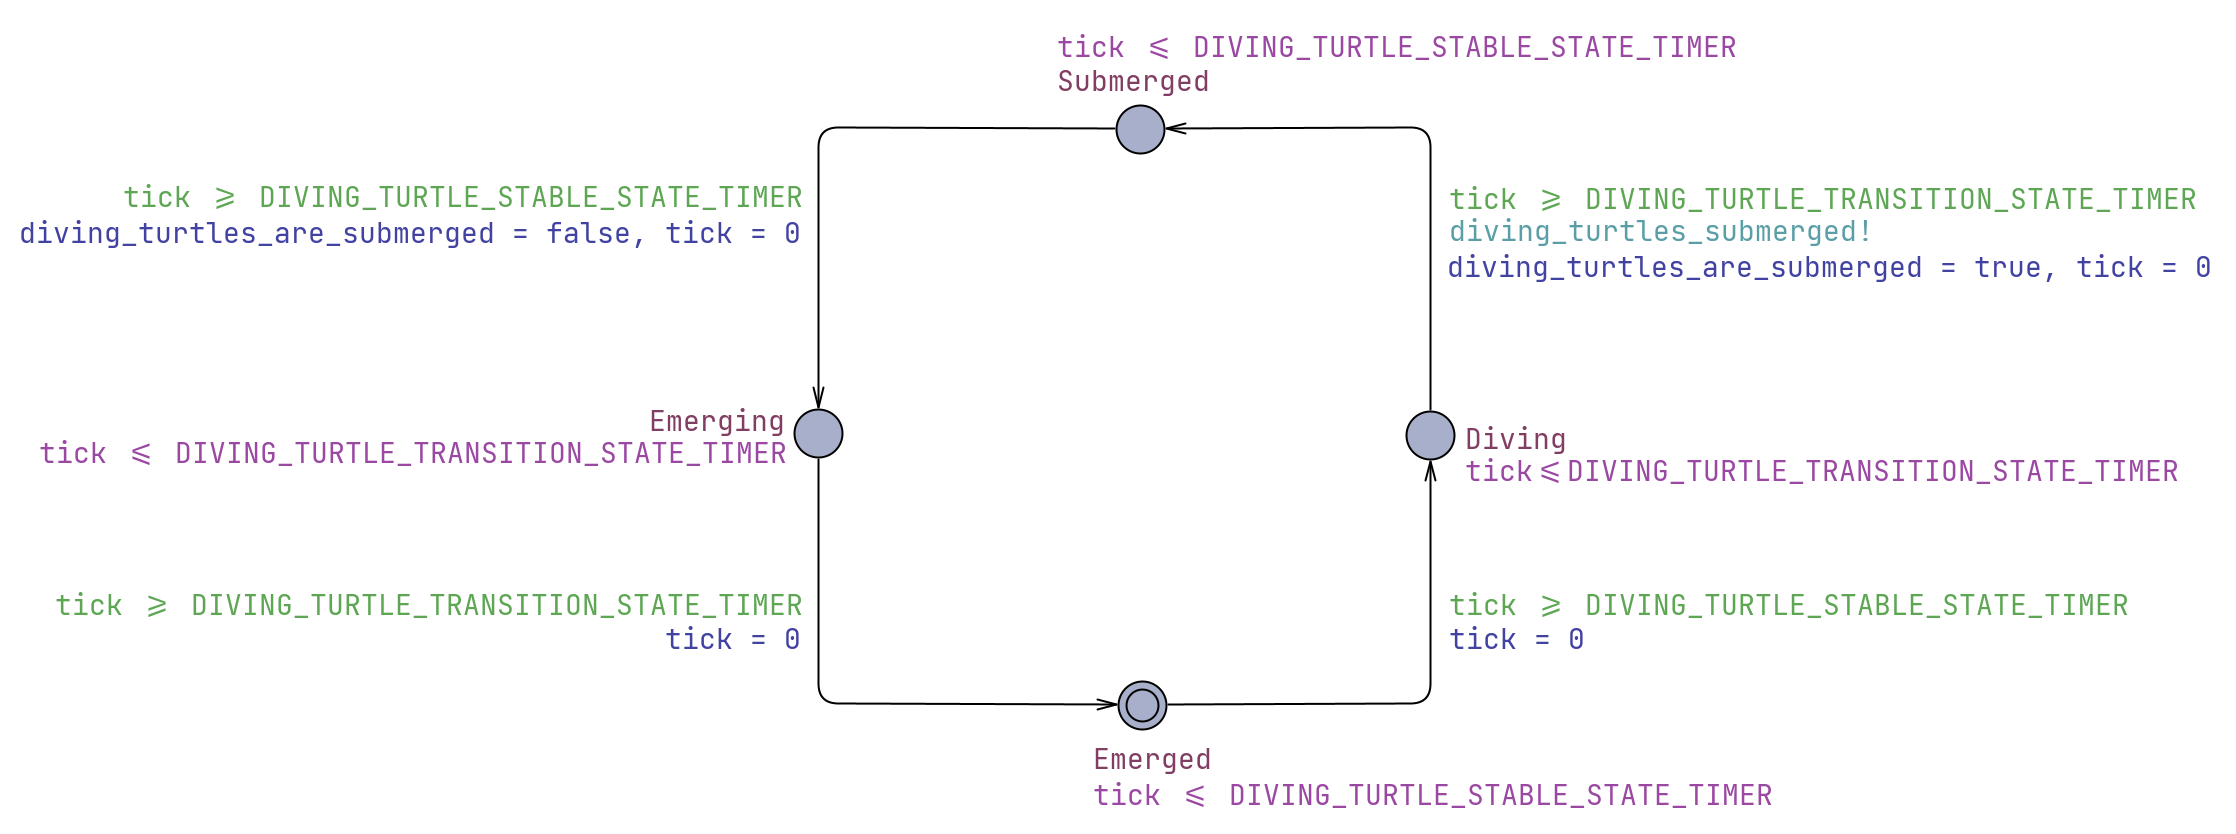
\includegraphics[width=\textwidth]{images/diving_turtles_cycle.png}
    \caption{Diving Turtles Manager Template}
    \label{fig:divingTurtlesImage}
\end{figure}

\subsection{Channels}
The communication between templates relies on three synchronisation channels, 
each chosen as broadcast or binary according to how many automata must react 
to the event:
\begin{itemize}
    \item \texttt{kill\_frog} (binary): requests the death of Frogger. It is 
    sent by a \textbf{VehicleLane} when a vehicle overlaps the frog, or by a 
    \textbf{FloatingLane} when the frog is on unsafe water or on a submerged 
    diving-turtle group. It is received only by the \textbf{Frogger} automaton, 
    which removes one life and respawns the frog.
    
    \item \texttt{frog\_moved} (broadcast): announces that Frogger has 
    completed a movement step. It is received by the \textbf{VehicleLane} and 
    \textbf{FloatingLane} templates, so that the current lane where Frogger is standing can check whether the 
    new position is unsafe; if so it signals the death through the \texttt{kill\_frog} channel. 
    It is broadcast because a priori is unkown which lane is interested in the message.
    
    \item \texttt{diving\_turtles\_submerged} (broadcast): announces that the 
    diving turtles have entered the submerged phase. It is sent by the 
    \textbf{Diving Turtle Manager} and received by the \textbf{FloatingLane} 
    templates containing diving turtles, which then check whether Frogger is 
    standing on a submerged turtle.
\end{itemize}


\subsection{Stochastic Variation}

\newpage
\section{Properties Verification}
In this section are shown the proprieties that have been checked over the system to be sure that
it behaves as expected and the queries requested are verified. 
The properties we discuss here can be found as queries in the Verifier section of UPPAAL.
Details about the time and RAM usage of the verification process can be found in the report.


\subsection{System verification}

\subsubsection*{A home bay is reachable}
\[ (\textrm{III}) : \quad \exists \Diamond \; \big( \textit{frog\_y} = 12 
   \;\wedge\; home\_bays[frog\_x] = 1 \big) \]
It's saying that exists at least one path that eventually will lead to 
Frogger reaching a home bay cell, i.e. a cell in row 12 whose column is 
marked as a home bay in the map.

\subsubsection{Frog is never alive on a vehicle cell}

\subsection{Properties Verification}
The following properties are expressed in TCTL, a simplified version is used in UPPAAL for the formal verification. 
Each property is briefly commented to explain its meaning with respect to the system behavior.

\subsubsection*{Absence of deadlock (without Frogger)}
\[ (\textrm{I}) : \quad \forall \square \; \neg\, \textit{deadlock} \]
Verified on the system without the Frogger automaton, this property states that 
along every path the model never reaches a deadlock state, i.e. the lanes and 
the diving-turtle cycle can always progress.

\subsubsection*{All vehicles and floating objects can only move inside their predefined row}
\[ (\textrm{II}) : \quad \forall \square \; \big( \forall i \;\; 
   \textit{L}[i].\textit{row} = i \big) \]
This property states that each vehicle and each floating object remains within 
its predefined row and never changes lane. It holds by construction, since the 
lane templates do not include any transition that would allow an object to move 
vertically.

Nonetheless, it can still be explicitly modelled as ``the lane never changes 
its row'' and verified, in order to confirm that no unexpected behaviour causes 
an object to leave its lane.

\subsubsection*{Frogger can reach the home bay in position (0,12)–(1,12)}
\[ (\textrm{III}) : \quad \exists \Diamond \; \big( \textit{frog\_y} = 12 
   \;\wedge\; home\_bays[0] = true \big) \]
It's saying that exists at least one path that eventually will lead to 
Frogger reaching a home bay cell, i.e. a cell in row 12 whose column is 
marked as a home bay in the map.

\subsubsection*{Frogger can score 17 points reaching the home bay in position (8,12)–(9,12)}
\[ (\textrm{IV}) : \quad \exists \Diamond \; \big(  home\_bays[3] = true 
   \;\wedge\; \textit{frog\_y} = 12 \;\wedge\; \textit{score} = 17 \big) \]
A refinement of the previous property: there exists a path on which Frogger 
reaches the home bay at $(8,12)$--$(9,12)$ while holding exactly 17 points.

\subsubsection*{Frogger can reach a yellow cell in row 6 after the player has lost two lives}
\[ (\textrm{V}) : \quad \exists \Diamond \; \big( \textit{frog\_y} = 6 
   \;\wedge\; \textit{lives} = \textit{MAX\_LIVES} - 2 \big) \]
There exists a path on which Frogger reaches a cell in row 6 (the safe median) 
after having lost exactly two lives, i.e. with three of the initial five 
remaining.

\subsubsection*{Frogger may stand on a log (with five lives) 10 seconds after the game starts}
\[ (\textrm{VI}) : \quad \exists \Diamond \; \big( \textit{lives} = 
   \textit{MAX\_LIVES} \;\wedge\; \textit{LANE\_STRUCTURES}[\textit{frog\_y}]
   [\textit{frog\_x}] = L \;\wedge\; \textit{frog\_timer} = 100 \big) \]
There exists a path on which, within 10 seconds from the start (100 ticks, 
since one tick is 0.1 s) and still with all five lives, Frogger is standing on 
a log.

\subsubsection*{Frogger can die riding a diving turtle that transitions to the submerged state}
\[ (\textrm{VII}) : \quad \exists \Diamond \; \big( 
   \textit{diving\_turtles\_are\_submerged} \;\wedge\; 
   \textit{frog\_on\_diving\_turtle} \big) \]
There exists a path on which Frogger is standing on a diving-turtle group at 
the moment it enters the submerged phase, which causes the cell to become open 
water and the frog to drown. This checks the interaction between the 
\textbf{DivingTurtleCycle} and the \textbf{FloatingLane} through the 
\texttt{diving\_turtles\_submerged} channel.

\subsection{Stochastic Verification}

\newpage
\section{Conclusion}
To summarize, we modelled and formally verified a simplified version of 
Frogger in UPPAAL, developing both a symbolic and a stochastic version of the 
system as a network of Timed Automata that captures all the core mechanics of 
the game. We verified a set of TCTL properties, proving 
both the correctness of the system and the reachability of requested queries. 
The work highlighted some design trade-offs adopted to avoid 
the state space explosion during verification, keeping the final model compact 
and efficient while preserving a faithful representation of the game logic.

\end{document}